%!TEX root = ../dokumentation.tex

\subsection{Client-Server}
\label{sec:Client-Server}
% Client-Server-Bild
Die Kommunikation in \acs{Redis} funktioniert nach dem \textit{Client-Server-Modell}.
Dieses Architektur funktioniert, wie in \autoref{fig:Client-Server} dargestellt.
Es gibt mehrere Clients, die mit einem Server kommunizieren. 
Clients selbst können jedoch nicht direkt miteinander kommunizieren.
Dementsprechend läuft jegliche Kommunikation immer über den Server.
Der Server erhält Nachrichten beziehungsweise Befehle von den \acs{Redis}-Clients und verarbeitet diese. 
Je nach Anfrage sendet der Server dann die entsprechende Antwort zurück an einen Client oder mehrere Clients gleichzeitig.
\begin{figure}[h]
    \centering
	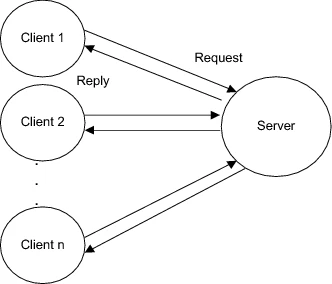
\includegraphics[width=0.48\textwidth]{images/Client-Server.png}
	\caption{\textit{Client-Server-Modell} (vgl. \cite{Bengel2014}, S.23)}
	\label{fig:Client-Server}
\end{figure}

Das besondere der \acs{Redis}-Architektur ist, dass es in verteilten \acs{Redis}-Systemen nicht nur einen, sondern mehrere Server geben kann.



